%%% template.tex
%%%
%%% This LaTeX source document can be used as the basis for your technical
%%% paper or abstract. Regardless of the length of your document, the commands
%%% are all the same.
%%% 
%%% The "\documentclass" command is the first command in your file. If you want to 
%%% prepare a version of your article with line numbers - a "review" version - 
%%% include the "review" parameter:
%%%    \documentclass[review]{acmsiggraph}
%%%

\documentclass{acmsiggraph}
\usepackage{amsmath}
\usepackage{amsfonts}
\usepackage{mathtools}
\usepackage{amssymb}
\usepackage{amsthm}
\usepackage{tikz}
\newcommand{\B}{\mathbb{B}} % binary set
\newcommand{\N}{\mathbb{N}} % set of natural numbers
\newcommand{\Z}{\mathbb{Z}} % set of integers 
\newcommand{\Q}{\mathbb{Q}} % set of rationals
\newcommand{\R}{\mathbb{R}} % set of reals
\newcommand{\C}{\mathbb{C}} % set of complex
\newcommand{\set}[1]{\left\{#1\right\}} % set, general

\title{Mathematical Mesh Generation}

\author{J\'{o}n Steinn El\'{i}asson\thanks{e-mail:jonsteinn@gmail.com}\\Reykjav\'{i}k University}
\pdfauthor{Stephen N. Spencer}

\TOGonlineid{45678}

\keywords{Mesh, Functions}

\begin{document}

 \teaser{
   \captionsetup{type=figure}
   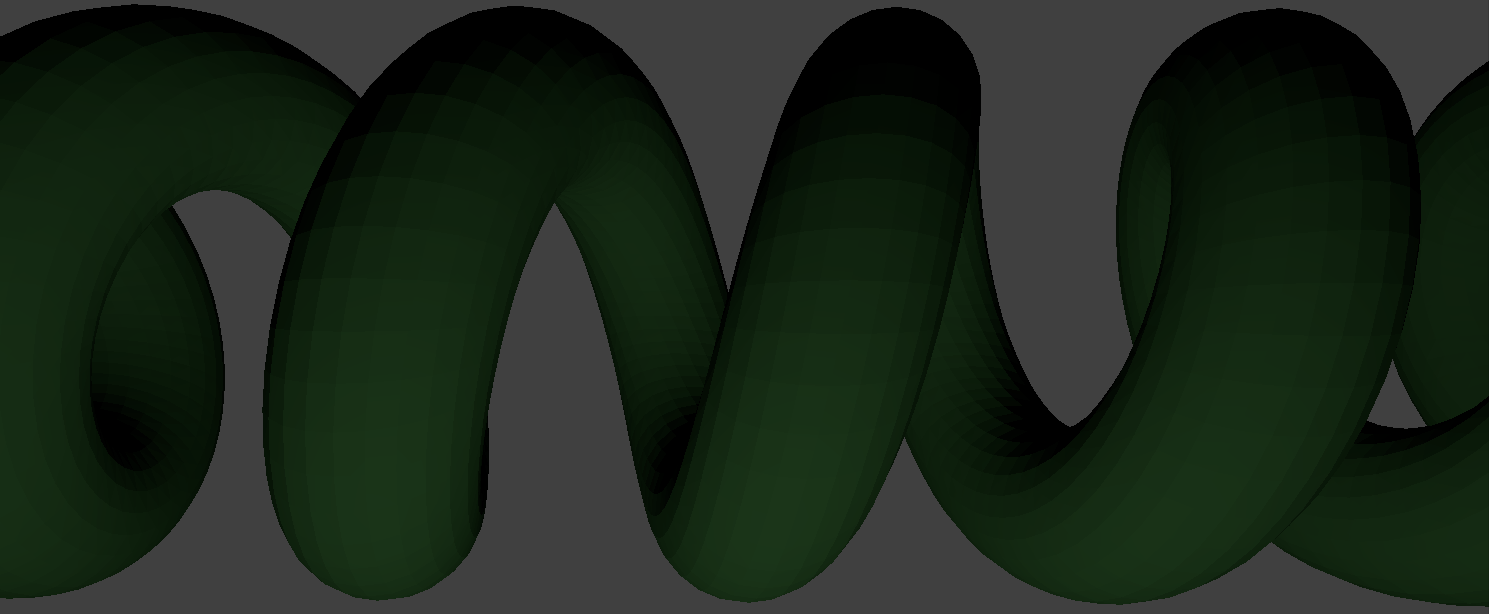
\includegraphics[height=1.5in]{images/spiral.png}
   \caption{A spiral mesh, rendered in Blender}
 }

\maketitle

\begin{abstract}

With mathematical functions we can map two dimensional planes into three dimensional surfaces to create some beautiful geometries. I created a web application, using Flask and WebGL, to create, preview and export the resulting three dimensional surfaces of such mappings. Thereupon they can be imported to any system supporting the format for further use.

\end{abstract}

\keywordlist

\section{Motivation}
Prior year's particle exporters sparked the idea of some kind of export system but I did want to create something different. I thought it would be a fun project to create objects with mathematics. It would allow countless possibilities for the user to create various things.

The most obvious use for such a system is to visualize mathematical functions where we can roam freely and explore the result of the mapping. Many game engines offer predefined primitive objects like spheres and we can add further objects to that, like toruses, cones or pyramids. It can also be used to generate terrain like surfaces.

\section{Related work}
Many of the computer algebra systems out there support 3D plots such as \href{https://www.wolfram.com/mathematica/}{Wolfram Mathematica} and \href{http://www.sagemath.org/}{SageMath}. They are usually somewhat limited when exploring these objects and often only allow rotation and zooming and you mostly feel like you have a 3D object on a paper rather than being in 3D space with the object. I have not found one that support mesh exporting since that is usually not what they are intended for.


\section{Approach}
\subsection{User interface}
The interface is written in javascript and html. It offers the user three ways of creating meshes using various parameters, view what he has created and download it. I originally intended to create the project in Unity but did not find a suitable way to convert input into functions. Creating a web application was mostly just a means to an end and as little effort as possible was placed into that part of the project.

\subsection{Preview rendering}
I used a WebGL library called Three.js to render a preview of any object created. The scene is potentially kept raw and only includes the object it self, which is loaded from the \texttt{.obj} file created, a camera and lights. There is an ambient light and a point light that follows the camera. To explore this primitive world, there are key events to translate and rotate the camera.

\subsection{Calculations}
There are two types of mappings available to generate meshes. The method of generating a mesh works mostly the same for all mappings.
\begin{itemize}
\item A mapping from $\R^2 \to \R^3$ where 2D points of a grid in the $xz$-plane are mapped to height point. We can either map with a defined function or using noise.
\item A mapping from $\R^2 \to \R^3$ where 2D points of a grid ($uv$-plane, unrelated to our space) are mapped to a 3D point.
\end{itemize} 
Here we will go through the process of generating a mesh using a function from $\R^2$ to $\R^3$. We begin by parsing the input according to our supported syntax and convert it to a lambda function which is used to map our 2D points to a height point

If the user asks for a $n_x \times n_z$ grid with $x_a \leq x \leq x_b$ and $z_a \leq z \leq z_b$, then each cell is of size $\Delta x \cdot \Delta z$ where $\Delta x = \frac{x_b-x_a}{n_x}$ and $\Delta z = \frac{z_b-z_a}{n_z}$. We take each cell in the grid and find the height for all of its vertices.

\begin{figure}[ht]
  \centering
  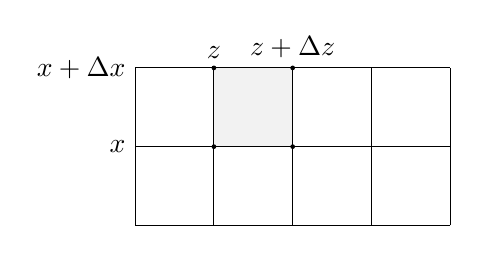
\begin{tikzpicture}
    \fill[gray!10] (1,1) rectangle (2,2);
    \draw (0,0) grid (4,2);
    \fill (1,1) circle (0.03);
    \fill (1,2) circle (0.03);
    \fill (2,1) circle (0.03);
    \fill (2,2) circle (0.03);
    \draw (0,1) node[left] {$x$};
    \draw (0,2) node[left] {$x+\Delta x$};
    \draw (1,2) node[above] {$z$};
    \draw (2,2) node[above] {$z+\Delta z$};
  \end{tikzpicture}
  \caption{A single cell in a grid}
  \label{fig:cell}
\end{figure}

Each cell is then split into two triangles, $(031)$ and $(023)$ as shown in figure \ref{fig:tri}. For the triangle $(031)$ we use the cross product of the vectors $(31)$ and $(30)$ as normal and the cross product of $(02)$ and $(03)$ for $(023)$.

\begin{figure}[ht]
  \centering
  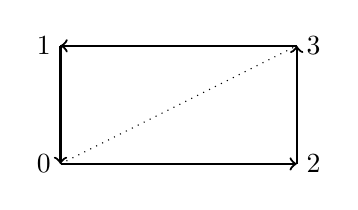
\begin{tikzpicture}
  	\draw (0,0) rectangle (3,1.5);
    \draw[dotted] (0,0) -- (3,1.5);
    \draw (0,0) node [left] {$0$};
    \draw (0,1.5) node [left] {$1$};
    \draw (3,0) node [right] {$2$};
    \draw (3,1.5) node [right] {$3$};
    \draw[thick,->] (3,1.5) -- (0,1.5);
    \draw[thick,->] (0,1.5) -- (0,0);
    \draw[thick,->] (0,0) -- (3,0);
    \draw[thick,->] (3,0) -- (3,1.5);
  \end{tikzpicture}
  \caption{Vertices, triangles and vectors}
  \label{fig:tri}
\end{figure}

All of these results are written to an \texttt{.obj} file along with texture coordinates which are by default, just a scaling of our domain into the texture coordinate plane. 

The only difference for the noise mesh is that the height map is a random noise function and for the parametric surfaces, we have three functions and must map all three coordinates of each point.

\subsection{Texture coordinates}
Since we are just generating a file and not directly using a rendering pipeline (other than the preview one), there are limited options for textures. I spent quite some time experimenting with texture coordinates to deal with the difference of triangle areas. By generating enough triangles you shouldn't see any stretched texture on the object but that isn't a good way to avoid the problem since the detailed meshes can be expensive.

Near the end of the project, I got the idea to calculate the length of each line (both horizontal and vertical) in the grid after it had been mapped to a 3D surface and use them to get better texture coordinates. Two such grid lines can be seen highlighted in the grid in figure \ref{fig:glines}. 
\begin{figure}[ht]
  \centering
  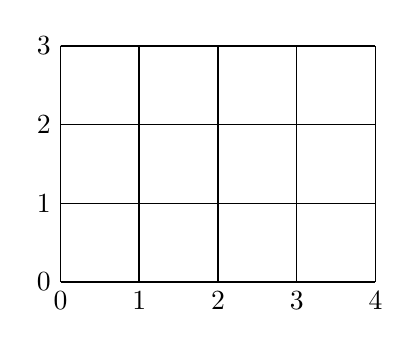
\begin{tikzpicture}
    \draw (0,0) grid (4,3);
    \foreach \x in {0,1,2,3} {
    	\draw (0,\x) node[left] {$\x$};
        \draw (\x,0) node[below] {$\x$};
        \draw[thick] (1,0) -- (1,3);
        \draw[thick] (0,3) -- (4,3);
    }
    \draw (4,0) node [below] {$4$};
  \end{tikzpicture}
  \caption{Grid lines}
  \label{fig:glines}
\end{figure}
For each point $(n,k)$ on the grid, we take the texture coordinate of $(n-1,k)$ and add to it 
\begin{align*}
\frac{\text{dist}((n,f(n,k),k),(n-1,f(n-1,k),k))}{\text{length of $z=k$ after being mapped}}
\end{align*}
which gives us the $u$ coordinate for $(n,k)$. The $v$ coordinate is obtained similarly. An example texture map of this procedure can be seen in figure \ref{fig:uvmap}.

\begin{figure}[ht]
  \centering
   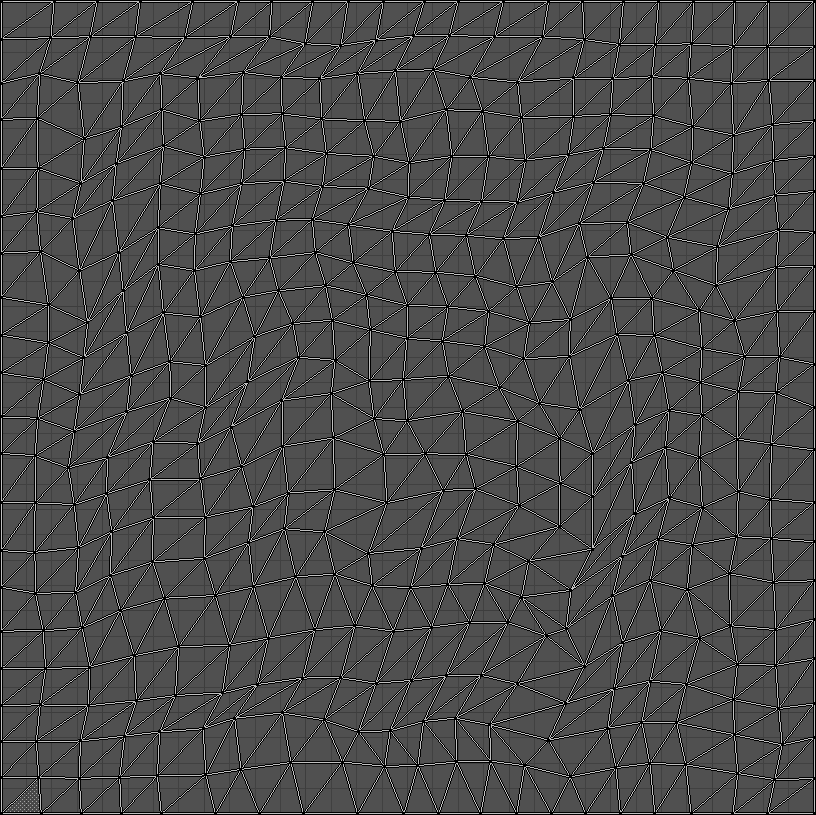
\includegraphics[width=2in]{images/uvmap.png}
  \caption{Length based texture coordinates}
  \label{fig:uvmap}
\end{figure}

\section{Results}
All the maps work as intended but they are generated based on input so there are of course ways to get an
incorrect visualization of a function, for example by using a small grid (in terms of cells) for a rapidly changing function on a large intervals. Figure \ref{fig:dini} shows an example from the preview scene.

\begin{figure}[ht]
  \centering
   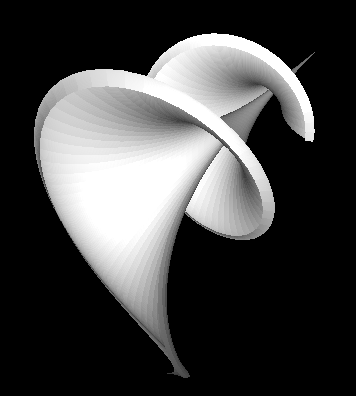
\includegraphics[width=2in]{images/dinis.png}
  \caption{Dini's surface}
  \label{fig:dini}
\end{figure}

We can download the mesh in Waterfront's \texttt{.obj} file format and import it to Blender or anything that supports the it. To use it in Unity for example, the file needs to be converted to a \texttt{.fbx} format and there are numerous converters available.

The length based texture coordinates can bee seen in figure \ref{fig:lentex}. They avoid triangles with stretched textures and play out quite nicely.

\begin{figure}[ht]
  \centering
   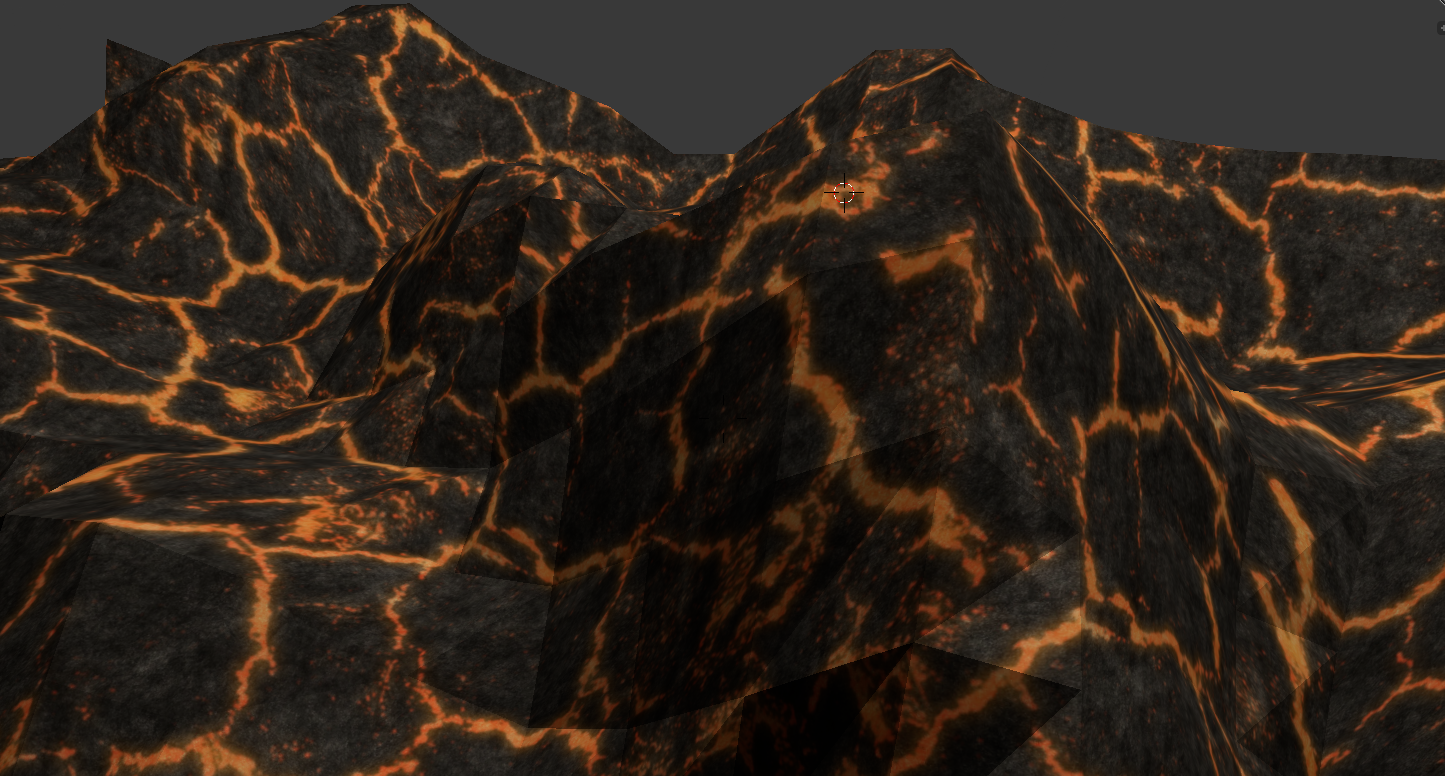
\includegraphics[width=3in]{images/texture.png}
  \caption{Length based texture mapping}
  \label{fig:lentex}
\end{figure}

There is however a flaw in this method that can occur. In texture coordinates, each cell can end up being mapped to a \href{https://en.wikipedia.org/wiki/Concave_polygon}{concave polygon} rather than a \href{https://en.wikipedia.org/wiki/Convex_polygon}{convex} which means that the triangles we split the cell into could potentially overlap. This is shown in figure \ref{fig:flaw}.

\begin{figure}[ht]
  \centering
  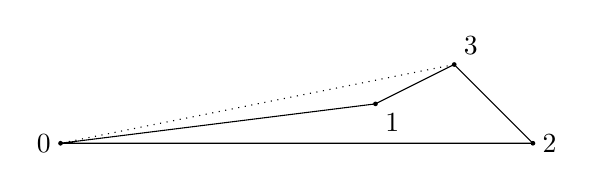
\begin{tikzpicture}
  	\draw (0,0) -- (4,0.5) -- (5,1) -- (6,0) -- (0,0);
    \fill (0,0) circle (0.03) node[left] {$0$};
    \fill (4,0.5) circle (0.03) node[below right] {$1$};
    \fill (5,1) circle (0.03) node[above right] {$3$};
    \fill (6,0) circle (0.03) node[right] {$2$};
    \draw[dotted] (5,1) -- (0,0);
  \end{tikzpicture}
  \caption{Flaw in length based texture coordinates}
  \label{fig:flaw}
\end{figure}

An approach that might fix this is to split the cell from $(1)$ to $(2)$ when this occurs. We can guarantee that $(1)$ and $(0)$ are to the left of $(3)$ and $(2)$ respectively, and  that $(1)$ and $(3)$ are above $(0)$ and $(2)$. I think each cell should always be able to pick either a split from $(03)$ or $(12)$ that does not go outside the cell but that would make the file generating a lot more complicated and is left for future work.

\section{Future work}
The code needs a lot of clean up, both performance and style wise and if this were to be a web application, there are some additional security issues that need to be handled.

Having some shaders available for the WebGL preview would be a nice touch or even support uploading them.

The length based coordinates are a nice idea and would work if we were drawing rectangles rather than triangles. Is this approach possible with triangles? That is the next step of this project.

%\bibliographystyle{acmsiggraph}
%\nocite{*}
%\bibliography{template}
\end{document}
